\documentclass{article}
\usepackage{xeCJK}
\usepackage{amsmath,esint,amssymb,amsthm}
\usepackage{hyperref}
\usepackage{pstricks-add}
\usepackage[bottom]{footmisc}
\setCJKmainfont[AutoFakeBold]{SimSun}
\usepackage{bm}
\def\v#1{\overrightarrow{#1}}
\begin{document}
\title{笔记整理}
\author{赵丰}
\maketitle
\tableofcontents
\section{第二周第二次课}
\newglossaryentry{pathlines}
{
  name=迹线,
  description={某一流体质点的运动轨迹}
}
\textbf{\gls{pathlines}}

某一流体质点的运动轨迹,其轨迹方程为常微分方程组$\frac{d \v{x}}{d t}=\v{v}$,
$\v{x}$为流体质点在$t$时刻的位置,同时也依赖于初始位置$\v{x_0}$(常微分方程组初值);$\v{v}=u\v{i}+v\v{j}+w\v{k}$为速度场,
每个分量都是空间位置和时间$t$的函数,
常微分方程组写成分量的形式为:
\begin{equation}\label{eq:22tr}
\begin{cases}
\frac{dx}{dt}=&u(x,y,z,t)\\
\frac{dy}{dt}=&v(x,y,z,t)\\
\frac{dz}{dt}=&w(x,y,z,t)
\end{cases}
\end{equation}
如对于如下的速度场
\begin{equation}\label{eq:w220}
(u,v,w)=(\frac{x}{1+t},y,z)
\end{equation}
$t=0$时初值条件为$(x,y,z)=(1,1,1)$,可直接求出上述常微分方程(ODE)有唯一解:
\begin{equation}
\begin{cases}
x=&1+t\\
y=&e^t\\
z=&1
\end{cases}
\end{equation}
这是关于$t$的参数曲线,可以通过消元得到$y=e^{x-1},z=1$,这是用空间两个曲面的交线表示曲线的方法。

\newglossaryentry{streamlines}
{
  name=流线,
  description={曲线上每点的切线方向与该点的速度场方向一致}
}
\textbf{\gls{streamlines}}

数学定义为
\begin{equation}
\frac{d \v{x}(s)}{d s}\times \v{v} =\v{0}
\end{equation}
上述定义在给定速度场后描述了空间这样一簇曲线,每条曲线每点的切线方向与该点的速度场方向一致。
使用向量外积的定义得到等价的定义形式
\begin{equation}\label{eq:2222st}
\frac{dx}{u(x,y,z,t)}=\frac{dy}{v(x,y,z,t)}=\frac{dz}{w(x,y,z,t)}
\end{equation}
这里时间$t$是常数。
上述方程如取$x$为自变量,可得到关于$(y(x),z(x))$的常微分方程组。
比如对$t=0$时刻\eqref{eq:w220}式给出的速度场为$(u,v,w)=(x,y,z)$,求过$(1,1,1)$点的流线即解ODE:
\begin{equation}
\begin{cases}
\frac{dy}{dx}=&\frac{y}{x}\\
\frac{dz}{dx}=&\frac{z}{x}
\end{cases}
\end{equation}
初值条件是$y(1)=1,z(1)=1$,从而有唯一解$y=x,z=x$。
可以看出,对同一个流场,流线和迹线是不同的。

但对于定常流,即$\bm{v}$不随时间变化,流线簇和迹线簇重合。比如考虑平面流场$(u,v)=(ax,-ay)$,
\eqref{eq:22tr}给出曲线簇$x=c_1e^{at},y=c_2e^{-at}$,\eqref{eq:2222st}给出曲线簇$xy=c$,它们表示同一曲线簇。

其他概念:

脉线、时间线、流管、流体线、流体面

\textbf{流体微团}


考虑一流体微团(系统)研究其变形规律:
\begin{figure}[!ht]
\def\svgwidth{8cm}
\centering
\input{deformation.eps_tex}
\caption{xz平面矩形的变形}\label{fig:221}
\end{figure}
由图\ref{fig:221}可以看到,$\v{OO'}+\v{O'B'}=\v{OB}+\v{BB'}$,
所以
\begin{align}\label{eq:22221}
\v{O'B'}=&\v{OB}+\v{BB'}-\v{OO'}\nonumber\\
=&\Delta x \v{i}+\v{v_B}\Delta t - \v{v_O} \Delta t
\end{align}
又
\begin{align*}
\v{v_B}=&\v{v}(x+\Delta x,y,z,t)\\
\v{v_O}=&\v{v}(x,y,z,t)
\end{align*}
所以\eqref{eq:22221}式化为:
\begin{equation}
\v{O'B'}=\Delta x \v{i} + \Delta x\Delta t \frac{\partial \v{v}}{\partial x}
\end{equation}
进一步设速度场$\v{v}=(u,v,w)$,则上式在直角坐标系下为:
\begin{equation}\label{eq:222}
\v{O'B'}=[(1+\frac{\partial u}{\partial x}\Delta t)\v{i}+\frac{\partial v}{\partial x}\Delta t\v{j}+\frac{\partial w}{\partial x}\Delta t\v{k}]\Delta x
\end{equation}
同样的方法可求出$\v{C'D'}$:
\begin{align*}
\v{C'D'}=&\v{CD}+\v{DD'}-\v{CC'}\\
=&\Delta x\v{i}+[\v{v}(x+\Delta x,y,z+\Delta z,t)-\v{v}(x,y,z+\Delta z,t)]\Delta t\\
=&\Delta x \v{i} +  \Delta x\Delta t \frac{\partial \v{v}}{\partial x}\\
\Rightarrow & \v{O'B'}=\v{C'D'}
\end{align*}
所以正六面体流体微团的微小变形后仍是平行六面体,其变形后的体积可用平行六面体体积公式求得。

设变形前正六面体由自$O'$出发的向量$\v{OA}=\Delta y\v{j},\v{OB}=\Delta x \v{i},\v{OC}=\Delta z \v{k}$张成,
变形后的六面体由自$O'$出发的向量$\v{O'A'},\v{O'B'},\v{O'C'}$张成,
对$xy,yz$两个表面类似的分析可以得到与\eqref{eq:222}类似的式子:
\begin{align*}
\v{O'C'}=&[\frac{\partial u}{\partial z}\Delta t\v{i}+\frac{\partial v}{\partial z}\Delta t\v{j}+(1+\frac{\partial w}{\partial z}\Delta t\v{k})]\Delta z\\
\v{O'A'}=&[\frac{\partial u}{\partial y}\Delta t\v{i}+(1+\frac{\partial v}{\partial y}\Delta t\v{j})+\frac{\partial w}{\partial y}\Delta t\v{k}]\Delta y
\end{align*}
变形前正六面体体积$\Delta \tau (t)=\Delta x\Delta y\Delta z$,
经过$\Delta t$时间变形后六面体体积使用混合积公式\cite{mixedProduct}并略去高阶小为:
\begin{equation}
\Delta \tau (t+\Delta t)=[1+(\frac{\partial \v{u}}{\partial x}+\frac{\partial \v{v}}{\partial y}+\frac{\partial \v{w}}{\partial z})\Delta t]\Delta x\Delta y\Delta z
\end{equation}
定义流体微团的瞬时\textbf{体膨胀率}为单位体积变化的速率,即
\begin{equation}
\Delta \tau'(t)=\lim_{\Delta t \to 0} \frac{\Delta \tau (t+\Delta t)-\Delta \tau (t)}{\Delta \tau (t)\Delta t}
\end{equation}
于是可以得到体膨胀率为$\nabla \cdot \v{v}$,为速度场的散度。当速度场的散度处处为0时,流体为不可压缩流体,变形前后体积不变。

类似的有\textbf{线变形率}的定义,对于$x$方向为:
\begin{equation}
\lim_{\Delta t \to 0} \frac{|\v{O'B'}|-|\v{OB}|}{|\v{OB}|\Delta t}
\end{equation}
其中使用Taylor 近似从\eqref{eq:222}式出发有:$|\v{O'B'}|\approx (1+\frac{\partial u}{\partial x}\Delta t)\Delta x$
于是可以求得$x$方向的线变形率为$\frac{\partial u}{\partial x}$,进而得到体膨胀率为三个方向线变形率之和的结论。


\textbf{流体的旋转角度}

对于流体绕$y$轴的旋转角度定义为$\v{O'B'}$相对于$\v{OB}$转过的角度与$\v{O'C'}$相对于$\v{OC}$转过的角度的平均值。
由于转角$\alpha$很小,有近似$\tan \alpha\approx \alpha$,所以由\eqref{eq:222}式
\begin{align*}
\measuredangle \left< \v{O'B'},\v{OB} \right>=&\frac{\frac{\partial w}{\partial x}\Delta t}{1+\frac{\partial u}{\partial x}\Delta t}\\
\approx & \frac{\partial w}{\partial x}\Delta t (1-\frac{\partial u}{\partial x}\Delta t)
\end{align*}
略去二阶小$(\Delta t)^2$即得到图中的$\alpha_1=\frac{\partial w}{\partial x}$,
因为顺时针方向为负,所以转角为$-\alpha_1$。同理求出图中的$\alpha_2=\frac{\partial u}{\partial z}$
所以流体绕$y$轴的旋转角度为
\begin{align}
\omega_y=&\frac{\alpha_2-\alpha_1}{2\Delta t}\nonumber\\
=&\frac{1}{2}(\frac{\partial u}{\partial z}-\frac{\partial w}{\partial x})
\end{align}

\textbf{流体的角变形率}

对于流体在$xz$平面的角变形率:
\begin{align}
\epsilon_{xz}=&\frac{\alpha_2+\alpha_1}{2\Delta t}\nonumber\\
=&\frac{1}{2}(\frac{\partial u}{\partial z}+\frac{\partial w}{\partial x})
\end{align}
% $S(V)$是流体微团变形后的表面,由Stokes公式:
% \[
% DV=\iiint\limits_{V}(\nabla \cdot \bm{u}Dt) dV
% \]
% 变形后的新体积
% 随时间的变化为$\frac{Dv}{Dt}$,

\section{第三周第一次课}
%\textbf{并矢与几何矢表示}
%设$\v{a},\v{b}$是三维空间向量$,则$\v{a},\v{b}$的几何矢为$\v{a}\v{b}$,$\v{a},\v{b}$的外积为$\v{a}\wedge \v{b}$
\textbf{流动运动学常用物理量的张量表示}

变形率张量
$\bm{S}=[s_{ij}]=\frac{1}{2}\left(\Delta \v{v}+(\Delta \v{v})^{\mathrm{T}}\right)$,类似弹性力学中的应变张量,为二阶对称张量。
反称张量$\bm{\Omega}=[\Omega_{ij}]=[\epsilon_{ijk}\omega_k]$,其中$\omega=\frac{1}{2}\Delta \times \bm{v}$
并且我们有:
\begin{equation}\label{eq:w31AS}
\nabla \v{v}=\bm{S}-\bm{\Omega}\cite{velocityGradient}
\end{equation}
其中速度梯度张量 $\nabla \v{v}=[v_{ij}]=[\frac{\partial v_i}{\partial x_j}]$
\footnote{$\bm{\Omega}$前是减号不是加号}

\textbf{运动分析}

\begin{figure}[!ht]%I can not compile this pstricks figure on my pC
\centering
%LaTeX with PSTricks extensions
%%Creator: inkscape 0.92.2
%%Please note this file requires PSTricks extensions
%\documentclass{article}
%\pagestyle{empty}
%\usepackage{pstricks-add}
%\usepackage{tikz}
%\begin{document}
%\begin{figure}
%\begin{pspicture}(0,0)(5,5)
%spatial axis xyz
%\psline{->}(2,2)(2,4)
%\psline{->}(2,2)(4,2)
%\psline{->}(2,2)(1,1)
%\rput(2,4){$y$}
%\rput(4,2){$x$}
%\rput(1,1){$z$}
% fluid particle pos
%\psline{->}(2,2)(3.2,2.7)
%\psline{->}(3.2,2.7)(3.8,3)
%\rput[b](3.1,2.7){$O$}
%\rput[b](3.9,3){$A$}
%\rput[b](3.5,2.85){$\delta \v{x}$}
%\rput[b](2.6,2.35){$\v{x}$}
%\end{pspicture}
%\end{figure}

%rewrite the above picture command with tikz
 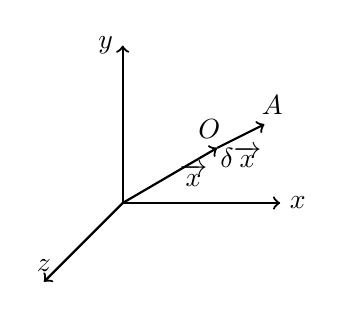
\begin{tikzpicture}
  \draw[thick,->] (2,2) -- (2,4);  
  \draw[thick,->] (2,2) -- (4,2);
  \draw[thick,->] (2,2) -- (1,1);
  \draw (2,4) node[anchor=east] {$y$};
  \draw (4,2) node[anchor=west] {$x$};
  \draw (1,1) node[anchor=south]{$z$};
  \draw (3.5,2.85) node[anchor=north] {$\delta \v{x}$};
  \draw (2.6,2.35) node[anchor=west] {$\v{x}$};
  \draw[thick,->] (2,2) -- (3.2,2.7);
  \draw[thick,->] (3.2,2.7) -- (3.8,3);
  \draw (3.1,2.7) node[anchor=south] {$O$};
  \draw (3.9,3) node[anchor=south]{$A$};
 \end{tikzpicture}
%\end{document}
\caption{流体质点从$O$点经$\Delta t$时间运动到$A$点}\label{fig:311}
\end{figure}

Helmholz 速度分解定理,参考图\ref{fig:311},有:
\begin{align}
\v{v_{A}} = & v_j(\v{x}+\delta \v{x},t)\v{e_j}\\
=& [v_j(\v{x},t)+\frac{\partial v_j}{\partial x_i}\delta x_i]\v{e_j}\\
=& [v_j(\v{x},t)+s_{ij}(\v{x},t)\delta x_i+\Omega_{ij}((\v{x},t))\delta x_i]\v{e_j}\,\footnotemark\\
=& \v{v_O} + \delta x \cdot \v{S_0} + \v{\omega_O}\times \delta \v{x}
\end{align}
\footnotetext{$\frac{\partial v_j}{\partial x_i}$是$v_{ji}$,与\eqref{eq:w31AS}不矛盾。}
其中最后一式用到了$\bm{\Omega}$和$\v{\omega}$的关系式:
\begin{equation}
\bm{\Omega} \v{x}= \v{\omega}\times \v{x} \cite{angularVelocityTensor}
\end{equation}

\newglossaryentry{vortex}
{
  name=涡量,
  description={速度场的旋量}
}
\textbf{\gls{vortex}}

定义为:$\v{\Omega}=\nabla \times \v{v}=2\v{\omega}$,其散度为零。

对于有相同流线方程的流场,其涡量场可以不同。比如流场
\begin{equation}\label{eq:31example}
\begin{cases}u=-y\\v=x\end{cases}(a) \begin{cases}u=-\frac{y}{x^2+y^2}\\v=\frac{x}{x^2+y^2}\end{cases}(b)
\end{equation}
二者的流线簇均为$x^2+y^2=c$,但$(a)$中涡量为$2\v{k}$
$(b)$中速度场在极坐标下为$\frac{\v{e_{\theta}}}{r}$,对于非原点处,
由极坐标系散度公式\cite{CylindricalCoordinates}得其散度为$\frac{\partial 1/r}{\partial \theta}=0$,
由极坐标系旋度公式\cite{CurlFormular}得涡量为$\v{0}$。
在原点处,由格林公式,速度的环量(环量积分)等于涡通量:
\begin{align}
\Gamma_l =& \oint_l \v{v}\cdot d\v{x}\\
=& \int_{0}^{2\pi} \frac{\v{e_{\theta}}}{r}\cdot  \v{e_{\theta}} rd\theta \\
=& 2\pi
\end{align}
另外不难验证$\arctan\frac{y}{x}$是后一个流场的势函数,在极坐标下其表示为$\theta$。

其他概念:

涡线、涡面、涡管

\begin{figure}[!ht]
\def\svgwidth{5cm}
\centering
\input{vortexIntensity.eps_tex}
\caption{涡通量的守恒性质}\label{fig:312}
\end{figure}



参考图\ref{fig:312},对于涡管的任一两个横截面$A_1,A_2$,有
\begin{equation}
\iint\limits_{A_1} \v{\Omega}\cdot \v{n_1} dA=\iint\limits_{A_2} \v{\Omega}\cdot \v{n_2} dA
\end{equation}
即沿涡管各截面涡通量大小相等。

\textbf{给定流场的散度与涡量求速度场}

已知区域$D$内的速度场$\v{v}$在区域内满足如下的偏微分方程(PDE):
\begin{equation}
\begin{cases}
\nabla \cdot \v{v} &=\theta (\v{x})\\
\nabla \times \v{v} &=\v{\Omega}(\v{x})\\
\end{cases}
\end{equation}
在边界上给出法向速度的大小:$\v{v}\cdot \v{n} =v_{bn}(\v{x})$
则由Poisson方程在Neumann边界条件下解的性质可以得到速度场是唯一确定的。


首先运用PDE的叠加原理将原问题分解为求如下三个PDE:
\begin{equation}\label{eq:311t3}
\begin{cases}
\nabla \cdot \v{v_E} &=\theta (\v{x})\\
\nabla \times \v{v_E} &=\v{0}\\
\end{cases}(a)
\begin{cases}
\nabla \cdot \v{v_V} &=0\\
\nabla \times \v{v_V} &=\v{\Omega}(\v{x})\\
\end{cases}(b)
\begin{cases}
\nabla \cdot \v{u} &=0\\
\nabla \times \v{u} &=\v{0}\\
\end{cases}(c)
\end{equation}
其中(\ref{eq:311t3}.c)式附加第二类边界条件$\v{u}\cdot \v{n} =v_{bn}(\v{x})-\v{v_E}\cdot \v{n}-\v{v_N}\cdot \v{n}$

对于(\ref{eq:311t3}.a),由无旋条件可知存在势场$\Phi_E$使得 $\v{v_E}=\nabla \Phi_E$,于是得到$\Phi_E$在求解区域内满足Poisson 方程:
\begin{equation}
\nabla^2 \Phi_E(\v{x})=\theta(\v{x})
\end{equation}
该方程可由三维Laplace方程的基本解$\frac{1}{|\v{x}|}$与$\theta(\v{x})$做卷积得到\cite{FundamentalSolution},写成分量的形式即为:
\begin{equation}\label{eq:31similar}
\Phi_E(x,y,z)=-\frac{1}{4\pi} \iiint\limits_D \frac{\theta(\xi,\eta,\zeta)}{R(x,y,z;\xi,\eta,\zeta)}d\xi d\eta d\zeta
\end{equation}
这里
\begin{align}
R(x,y,z;\xi,\eta,\zeta)=&|\v{R}((x,y,z;\xi,\eta,\zeta))|\\
\v{R}((x,y,z;\xi,\eta,\zeta))=&(x-\xi)\v{i}+(y-\eta)\v{j}+(z-\zeta)\v{k}
\end{align}
直接计算得到:$\nabla \frac{1}{R}=-\frac{\v{R}}{R^3}$,其中梯度算子是关于$(x,y,z)$的。
所以我们有:
\begin{equation}
\v{v_E}=\frac{1}{4\pi} \iiint\limits_D \frac{\theta(\xi,\eta,\zeta)\v{R}}{R^3}d\xi d\eta d\zeta
\end{equation}
比如散度场$\theta$为$\delta$函数,可以得到点源诱导的速度场为:
\begin{equation}
\v{v_E}=\frac{1}{4\pi} \frac{x\v{i}+y\v{j}+z\v{k}}{(x^2+y^2+z^2)^{3/2}}
\end{equation}
这与万有引力场和点电荷诱导的静电场形式相同。

对于(\ref{eq:311t3}.b),难以得到一般条件下的闭式解,因此对涡量$\Omega$在求解域的边界上附加条件
\begin{equation}\label{eq:31supp}
\v{\Omega}\cdot \v{n}=0
\end{equation}
为此,我们先用张量分析的$\epsilon-\delta$恒等式$\epsilon_{ilm}\epsilon_{ijm}=\delta_{jl}\delta_{mn}-\delta_{mj}\delta_{ln}$证明如下的等式:
\begin{equation}\label{eq:312times}
\nabla \times(\nabla \times \v{A})=\nabla(\nabla \cdot \v{A})-\nabla\cdot(\nabla \v{A})
\end{equation}
\begin{proof}
\begin{align*}
\nabla \times(\nabla \times \v{A}) =& \nabla (\epsilon_{ijk} \frac{\partial A_k}{\partial x_j} \v{e_i})\\
=&\epsilon_{nmi} \frac{\partial (\epsilon_{ijk} \frac{\partial A_k}{\partial x_j})}{\partial x_m} \v{e_n}\\
=&(\delta_{nj}\delta_{mk}-\delta{nk}\delta_{mj})\frac{\partial^2 A_k}{\partial x_j^2}\v{e_n}\footnotemark\\
=&(\frac{\partial^2 A_k}{\partial x_n^2}\v{e_n})-(\frac{\partial^2 A_n}{\partial x_j^2}\v{e_n})\\
=&(\frac{\partial}{\partial x_n}(\frac{\partial A_k}{\partial x_n})\v{e_n})-(\frac{\partial}{\partial x_k}(\frac{\partial A_n}{\partial x_j}\v{e_n}\v{e_j})\cdot \v{e_k})\\
=&(\frac{\partial}{\partial x_n}(\nabla\cdot \v{A})\v{e_n})-(\frac{\partial}{\partial x_j}(\nabla \v{A})\cdot \v{e_j})\\
=&\nabla(\nabla \cdot \v{A})-\nabla\cdot(\nabla \v{A})
\end{align*}
\footnotetext{$\frac{\partial^2 A_k}{\partial x_j^2}\v{e_n}$是对$A$的各个分量求Laplace,相当于对矢量$A$先求梯度再求散度。}
\end{proof}
运用上面的等式,我们推导 \textbf{Biot-Savart 定律}:

首先假设 (\ref{eq:311t3}.b) 中 $\v{v_V}$可以写成$\v{v_V}=\nabla \times \v{A}$,则(\ref{eq:311t3}.b)中第一式自然满足,而第二式由\eqref{eq:312times}式可化为:
\begin{equation}\label{eq:31AAA}
\nabla(\nabla \cdot \v{A})-\nabla\cdot(\nabla \v{A})=\v{\Omega}
\end{equation}
下面我们证明对于区域$D$,不考虑边界条件,\eqref{eq:31AAA}的一个解为:
\begin{equation}
\v{A}=\frac{1}{4\pi} \iiint\limits_D \frac{\v{\Omega}(\xi,\eta,\zeta)}{R(x,y,z;\xi,\eta,\zeta)} d\xi d\eta d\zeta
\end{equation}
\begin{proof}
首先证明$\nabla \cdot \v{A}=0$,记$\nabla$是关于$(x,y,z)$求梯度,而$\nabla'$是关于$\xi,\eta,\zeta$求梯度,于是有:
\begin{align*}
\nabla \cdot \v{A} =& \frac{1}{4\pi} \iiint\limits_D \v{\Omega}(\xi,\eta,\zeta)\cdot \nabla(\frac{1}{R}) d\xi d\eta d\zeta\\
=&-\frac{1}{4\pi} \iiint\limits_D \v{\Omega}(\xi,\eta,\zeta)\cdot \nabla'(\frac{1}{R}) d\xi d\eta d\zeta\\
=&-\frac{1}{4\pi} \iiint\limits_D \nabla'\cdot(\frac{\v{\Omega}}{R}) d\xi d\eta d\zeta \footnotemark\\
=&-\frac{1}{4\pi} \iint\limits_{\partial D} \frac{\v{\Omega}\cdot \v{n}}{R} dS\\
=&0\,\,(\text{由式}\eqref{eq:31supp})
\end{align*}
另一方面,与\eqref{eq:31similar}式类似,由基本解与$\Omega$做卷积得到:
\begin{equation}
-\nabla\cdot(\nabla \v{A})=\v{\Omega}
\end{equation}
从而我们得到了\eqref{eq:31AAA}式的一个特解。
\end{proof}
因此对于无散有旋的情形(\ref{eq:311t3}.b),我们得到速度场为:
\begin{align}
\v{v_V}=&\frac{1}{4\pi} \iiint\limits_D \nabla(\frac{1}{R}) \times \v{\Omega} d\xi d\eta d\zeta\\
=&\frac{1}{4\pi} \iiint\limits_D  \frac{\v{\Omega} \times \v{R}}{R^3}d\xi d\eta d\zeta \label{eq:31biotsavart}
\end{align}
以\textbf{直线涡诱导的速度场}为例,考虑一空间涡量场为:
\begin{equation}
\v{\Omega}\cdot \v{k}=\begin{cases}
\infty, & (0,0,z)\\
0, & \text{otherwise}
\end{cases}
\end{equation}
其余两个方向分量为零,并且涡通量为常数$\Gamma$,即对于区域$A_{\epsilon}(k)=\{(x,y,z)|x^2+y^2<\epsilon,z=k\}$,有
\begin{equation}
\iint\limits_{A_{\epsilon}(k)} \v{\Omega}\cdot \v{n} dS=\Gamma
\end{equation}
可以求出上述直线涡产生的速度场沿$z$轴方向不变,对于其$x,y$平面内的速度场,与式(\ref{eq:31example}.b)描述的相同。
下面用\eqref{eq:31biotsavart}式直接求该速度场,这里$D=\mathbb{R}^3$,代表全空间:
\begin{align*}
\v{v_V}=&\frac{1}{4\pi} \iiint\limits_D  \frac{\v{\Omega} \times \v{R}}{R^3}d\xi d\eta d\zeta, \,\,\text{化为累次积分,先算}\xi,\eta\\
=&\frac{1}{4\pi} \int_{\mathbb{R}}(\iint\limits_{A_{\epsilon}(\zeta)}\frac{\v{\Omega} \times \v{R}}{R^3}d\xi d\eta )d\zeta, \,\,\epsilon\text{ 可任意小}\\
=&\frac{1}{4\pi} \int_{\mathbb{R}}\left(\frac{\Gamma \v{k}\times \v{R'}}{R'^3}\right)d\zeta, R'=R(x,y,z;0,0,\zeta)\\
=&\frac{\Gamma}{4\pi} \int_{\mathbb{R}}\left(\frac{x\v{j}-y\v{i}}{(x^2+y^2+(z-\zeta)^2)^{\frac{3}{2}}}\right)d\zeta\\
=&\frac{\Gamma}{2\pi}\frac{-y\v{i}+x\v{j}}{x^2+y^2}\\
\end{align*}


\section{第四周第一次课}

针对式(\ref{eq:311t3}.c),结合附加的第二类边界条件,由无旋条件,
我们设$\v{u}=\nabla \phi$,则$\phi$满足Neumann边界条件的PDE:
\begin{equation}\label{eq:41t3}
\begin{cases}
\nabla ^2 \phi = & 0 \\
\frac{\partial \phi}{\partial \v{n}}|_{bn}= & v_{bn}(\v{x})-\v{v_E}\cdot \v{n}-\v{v_N}\cdot \v{n}\\
\end{cases}
\end{equation}
其中$\v{v_E},\v{v_N}$是(\ref{eq:311t3}.a),(\ref{eq:311t3}.b)的特解。
方程\eqref{eq:41t3}可以使用格林函数法求解\cite{GreenFunction},

\textbf{流体动力学积分型方程}

\textbf{质量体} 的边界是随时间变化的,而\textbf{控制体} 的边界是不变的。
\textbf{Reynolds 输运}定理是联系质量体和控制体的桥梁,可以把关于质量体的守恒定律轻松转化为关于控制体的守恒定律。
它的陈述为:某一质量体的某一物理量在某时刻的随体导数等于该时刻相同体积相同形状的控制体该物理量的局部导数与该物理量的通过
该控制体的表面输运量。

下面设物理量为$Q$,时刻为$t_0$, 用$D^*(t)$表示质量体,而用$D$表示$D^*(t_0)$,$\Sigma$表示$D$的边界曲面,$\v{v}$是流体速度场,$d\tau$表示体积微元。则有
\begin{equation}
\frac{D}{Dt}[\iiint\limits_{D^*(t)}Qd\tau]_{t=t_0}=\iiint\limits_{D}\frac{\partial Q}{\partial t} d\tau + \oiint\limits_{\Sigma} Q\v{v}\cdot\v{n}dA
\end{equation}

下面给出两种推导,
\begin{align*}
\frac{D}{Dt}[\iiint\limits_{D^*(t)}Q(\v{x},t)d\tau] = & \iiint\limits_{D^*(t)} \frac{D}{Dt}[Q(\v{x},t)d\tau] \\
= & \iiint\limits_{D^*(t)} [\frac{DQ}{Dt}d\tau+Q\frac{D(d\tau)}{Dt}] \\
= & \iiint\limits_{D^*(t)} [\frac{DQ}{Dt}+Q\nabla \cdot \v{v}]d\tau, \,\,\text{体膨胀率的定义}\\
= & \iiint\limits_{D^*(t)} [\frac{\partial Q}{\partial t} + \v{v} \cdot \nabla Q +Q \nabla \cdot \v{v} ] d\tau \\
= & \iiint\limits_{D} \frac{\partial Q}{\partial t}d\tau + \iiint\limits_{D^*(t)} \nabla\cdot(Q\v{v})d\tau\\
= & \iiint\limits_{D} \frac{\partial Q}{\partial t}d\tau + \oiint\limits_{\Sigma} Q\v{v}\cdot \v{n} dA, \,\,\text{Gauss 公式}
\end{align*}

另一个推导要结合图示和一些几何直观,如图\ref{fig:412}所示:

\begin{figure}[!ht]
\centering
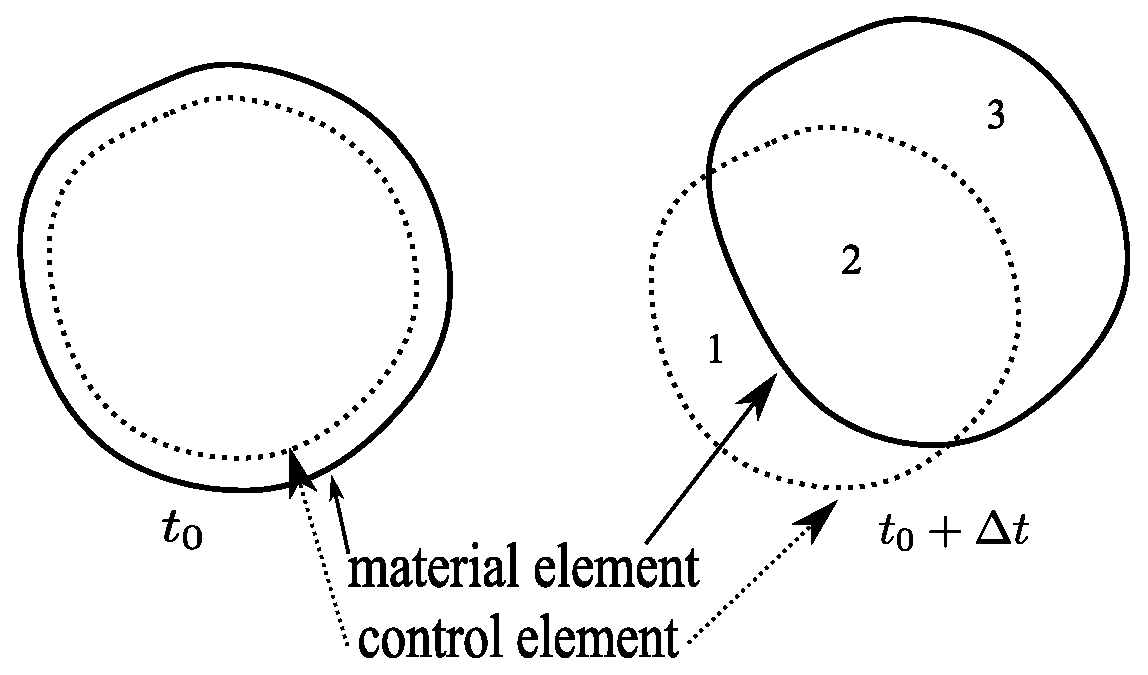
\includegraphics[width=5cm]{reynolds_derivation_illustration.eps}
\caption{雷诺输运方程推导图示}\label{fig:412}
\end{figure}
首先由随体导数的定义:
\begin{equation}
\frac{D}{Dt}[\iiint\limits_{D^*(t)}Qd\tau]_{t=t_0}=\lim_{\Delta t \to 0} \left[\frac{\iiint\limits_{D^*(t_0+\Delta t)}Q(\v{x},t_0+\Delta t) d\tau - \iiint\limits_{D^*(t_0)} Q(\v{x},t_0) d\tau  }{\Delta t}\right]
\end{equation}
积分区域$D^*(t_0+\Delta t)$可以写成$(1+2)+(3-1)$,数字所代表的区域如图\ref{fig:412}所示,注意到(1+2)仍表示控制体描述的区域,与$t_0$时刻相同,所以我们
进一步有:
\begin{align}\label{eq:41reynoldsD}
\frac{D}{Dt}[\iiint\limits_{D^*(t)}Qd\tau]_{t=t_0}=&\lim_{\Delta t \to 0} \left[
\frac{\iiint\limits_{D^*(t_0)}Q(\v{x},t_0+\Delta t) d\tau - \iiint\limits_{D^*(t_0)} Q(\v{x},t_0) d\tau  }{\Delta t}
\right]\nonumber\\
+&\lim_{\Delta t \to 0}\left[\frac{\iiint\limits_{D^*_3(t_0+\Delta t)}Q(\v{x},t_0+\Delta t) d\tau - \iiint\limits_{D^*_1(t_0+\Delta t)} Q(\v{x},t_0+\Delta t) d\tau  }{\Delta t}
\right]\nonumber\\
=& \iiint\limits_{D^*(t_0)}\frac{\partial Q}{\partial t} d\tau + \oiint\limits_{\Sigma} Q\v{v} \cdot \v{n} dA
\end{align}
式\eqref{eq:41reynoldsD}中第一项由于控制体的体积形状不变,所以对时间求导数可以挪到积分号里面;第二项根据问题的几何性质,
从1到3的体积变化由表面的流量引起,所以可以将体积的瞬时变化率转换为面积分的形式。

Reynolds 输运公式中取$Q$为不同的物理量,可以将Lagrange观点下的守恒方程(关于质量体)转化为Euler观点下的守恒方程(关于控制体)。

\textbf{质量守恒积分方程}:令$Q=$密度$\rho$,该守恒方程对任意坐标系均成立,对于质量体有:
\begin{equation}
\frac{D}{Dt} \iiint\limits_{D^*(t)}\rho d\tau =0
\end{equation}
应用Reynolds输运公式得到,对于控制体的质量守恒方程为
\begin{equation}\label{eq:41Conti}
\iiint\limits_{D}\frac{\partial \rho}{\partial t} d\tau = - \oiint\limits_{\Sigma} \rho \v{v}\cdot \v{n} dA
\end{equation}
即控制体内质量的变化等于从控制体表面流过的质量。

我们把质量守恒定律应用于定常流,即$\frac{\partial}{\partial t}=0$,从而得到
\begin{equation}
\oiint\limits_{\Sigma} \rho \v{v}\cdot \v{n} dA
\end{equation}
对于流管,其侧面密度流量为零,如下图所示:
\begin{figure}[!ht]
\def\svgwidth{5cm}
\centering
\input{streamTube.eps_tex}
\caption{定常流流管流量守恒的性质}\label{fig:41ST}
\end{figure}

我们有
\begin{equation}
\iint\limits_{A_1} \rho\v{v}\cdot \v{n_1} dA=-\iint\limits_{A_2} \rho\v{v}\cdot \v{n_2} dA
\end{equation}

若流动是均匀的,则有$\rho_1 v_{1n} A_1 = \rho_2 v_{2n} A_2$,其中 $v_{in}$表示面$A_i$法向的速度分量。


\textbf{动量守恒积分方程}:令$Q=\rho\v{v}$(矢量),
对于质量体,我们有
\begin{equation}
\frac{D}{Dt}\iiint\limits_{D^*(t)} \rho \v{v} d\tau = \iiint\limits_{D^*(t)} \rho \v{f} d\tau + 
\oiint\limits_{\Sigma^*(t)} \rho \v{T_n} dA
\end{equation}
应用Reynolds输运公式得到,对于控制体的动量守恒方程为

\begin{equation}\label{eq:41Momen}
\iiint\limits_{D}\frac{\partial (\rho\v{v})}{\partial t} d\tau = - \oiint\limits_{\Sigma} (\v{v}\cdot \v{n})\rho \v{v} dA +
\iiint\limits_{D^*(t)} \rho \v{f} d\tau + 
\oiint\limits_{\Sigma^*(t)} \rho \v{T_n} dA
\end{equation}

\textbf{动量矩守恒积分方程}:令$Q=\rho(\v{r} \times \v{v})$(矢量),
对于质量体,我们有
\begin{equation}
\frac{D}{Dt}\iiint\limits_{D^*(t)} \rho(\v{r} \times \v{v}) d\tau = \iiint\limits_{D^*(t)} \rho (\v{r}\times \v{f}) d\tau + 
\oiint\limits_{\Sigma^*(t)} \rho (\v{r} \times \v{T_n}) dA
\end{equation}
应用Reynolds输运公式得到,对于控制体的动量矩守恒方程为

\begin{equation}
\iiint\limits_{D}\frac{\partial}{\partial t}\rho(\v{r} \times \v{v}) d\tau = 
-\oiint\limits_{\Sigma^*(t)} \rho (\v{v} \cdot \v{n})\v{r} \times \v{v} dA+
 \iiint\limits_{D^*(t)} \rho (\v{r}\times \v{f}) d\tau + 
\oiint\limits_{\Sigma^*(t)} \rho (\v{r} \times \v{T_n}) dA
\end{equation}


\textbf{能量守恒积分方程}:令$Q=\rho(e+\frac{1}{2}|\v{v}|^2)$,$e$是单位质量流体的内能
\begin{equation}\label{eq:41Energy}
\frac{D}{Dt}\iiint\limits_{D^*(t)} \rho(e+\frac{1}{2}|\v{v}|^2) d\tau = \iiint\limits_{D^*(t)} \rho \v{f}\cdot\v{v} d\tau + 
\oiint\limits_{\Sigma^*(t)}  \v{T_n}\cdot\v{v} dA + \iiint\limits_{D^*(t)}\rho (\dot{q}+q_R)d\tau +
\oiint\limits_{\Sigma^*(t)} \lambda \v{n}\cdot \nabla T dA
\end{equation}
应用Reynolds输运公式即可将上述方程改写为控制体的形式,这里略去。

\section{第四周第二次课}

下面我们针对两组假设条件下的能量守恒积分方程进行化简:
第一组假设
\newglossaryentry{idealFluid}
{
  name=理想流体,
  description={表面力$T_n=-p \v{n}$}
}
\newglossaryentry{potentialField}
{
  name=有势场,
  description={存在标量函数$\Pi$, 使得$\v{f}=-\nabla \Pi$}
}
\newglossaryentry{steadyFlow}
{
  name=定常流,
  description={流体任意物理量$Q$只与空间坐标有关而与时间无关,满足$\frac{\partial Q}{\partial t}=0$}
}
\begin{itemize}
\item \gls{idealFluid},\glsdesc{idealFluid}
\item \gls{potentialField},\glsdesc{potentialField}
\item 绝热
\item \gls{steadyFlow},\glsdesc{steadyFlow}
\end{itemize}

在第一组假设下,能量守恒积分方程可化为
\begin{equation}\label{eq:42energy}
\oiint\limits_{\Sigma} \rho (e+\frac{1}{2}|\v{v}|^2)\v{v}\cdot\v{n} dA +
\iiint\limits_{D} \rho (\nabla \Pi)\cdot \v{v} d\tau 
+ \oiint\limits_{\Sigma} p \v{n}\cdot\v{v}dA=0
\end{equation}
我们尝试把上式第二项的体积分化为面积分,为此用到:
\begin{align*}
\rho (\nabla \Pi)\cdot \v{v} = & \nabla \cdot (\Pi \rho \v{v}) - \Pi \nabla \cdot(\rho \v{v})\\
= & \nabla \cdot (\Pi \rho \v{v}) \quad \text{定常流的连续性方程}
\end{align*}
因此我们得到
\begin{equation}
\oiint\limits_{\Sigma} \rho[\Pi + \frac{p}{\rho} + e + \frac{1}{2} |\v{v}|^2](\v{v}\cdot \v{n})dA=0
\end{equation}
上式中第一项$\Pi$表示体积势的贡献,第二项和第三项之和表示焓(内能与压力势之和),最后一项表示动能。

如果我们取$D$是一个流管,如图\ref{fig:412}所示,侧面积分为零,因此我们有
\begin{equation}
\oiint\limits_{A_1} \rho[\Pi + \frac{p}{\rho} + e + \frac{1}{2} |\v{v}|^2](\v{v}\cdot \v{n})dA=
-\oiint\limits_{A_2} \rho[\Pi + \frac{p}{\rho} + e + \frac{1}{2} |\v{v}|^2](\v{v}\cdot \v{n})dA
\end{equation}
假设面积$A_1,A_2$很小流动可以看作均匀的,从而
\begin{equation}
\rho[\Pi_1 + \frac{p_1}{\rho_1} + e_1 + \frac{1}{2} |\v{v_1}|^2](\v{v_1}\cdot \v{n_1})A_1=
-\rho[\Pi_2 + \frac{p_2}{\rho_2} + e_2 + \frac{1}{2} |\v{v_2}|^2](\v{v_2}\cdot \v{n_2})A_2
\end{equation}
代入微元流管的连续性方程
$\rho(\v{v}\cdot \v{n})A_1=-\rho(\v{v}\cdot \v{n})A_2$,我们得到
\begin{equation}
\Pi_1 + \frac{p_1}{\rho_1} + e_1 + \frac{1}{2} |\v{v_1}|^2 = \Pi_2 + \frac{p_2}{\rho_2} + e_2 + \frac{1}{2} |\v{v_2}|^2
\end{equation}
因此沿流线,我们得到第一组假设下的Bernoulli方程
\begin{equation}
\Pi + \frac{p}{\rho} + e + \frac{1}{2} |\v{v}|^2=c
\end{equation}
第二组假设
\newglossaryentry{uncompressibleCondition}
{
  name=不可压缩条件,
  description={流体微团体积不随时间变化,满足$\frac{D \rho}{D t}=0$}
}
\begin{itemize}
\item \gls{idealFluid}
\item \gls{potentialField}
\item \gls{uncompressibleCondition},\glsdesc{uncompressibleCondition}
\item \gls{steadyFlow}
\end{itemize}
在第二组假设下,由于体膨胀作功的部分为零,由热力学第一定律,内能的变化只与热交换有关,
因此在能量守恒方程中我们可以将内能与热交换项分离出来,从而得到\eqref{eq:42energy}式,但此时$e=0$,
类似的化简得到在第二组假设下的Bernoulli方程
\begin{equation}
\Pi + \frac{p}{\rho} + \frac{1}{2} |\v{v}|^2 = c
\end{equation}
进一步假设有势场是重力场,即$\Pi=gz$,$z$代表高度方向坐标,则得到Bernoulli方程的常用形式:
\begin{equation}
gz + \frac{p}{\rho} + \frac{1}{2} |\v{v}|^2 = c
\end{equation}

\begin{equation}
\end{equation}

\begin{thebibliography}{9}
\bibitem{mixedProduct} \href{https://en.wikipedia.org/wiki/Triple_product}{https://en.wikipedia.org/wiki/Triple\_product}
\bibitem{velocityGradient}\href{http://www.continuummechanics.org/velocitygradient.html}{http://www.continuummechanics.org/velocitygradient.html}
\bibitem{angularVelocityTensor}\href{https://en.wikipedia.org/wiki/Angular_velocity#Angular_velocity_tensor}{https://en.wikipedia.org/wiki/Angular\_velocity\#Angular\_velocity\_tensor}
\bibitem{CylindricalCoordinates}\href{https://en.wikipedia.org/wiki/Divergence#Cylindrical_coordinates}{https://en.wikipedia.org/wiki/Divergence\#Cylindrical\_coordinates}
\bibitem{CurlFormular}\href{https://en.wikipedia.org/wiki/Curl_(mathematics)}{https://en.wikipedia.org/wiki/Curl\_(mathematics)}
\bibitem{FundamentalSolution}\href{https://en.wikipedia.org/wiki/Fundamental_solution}{https://en.wikipedia.org/wiki/Fundamental\_solution}
\bibitem{GreenFunction}\href{https://en.wikipedia.org/wiki/Green\%27s_function#Green.27s_functions_for_the_Laplacian}{https://en.wikipedia.org/wiki/Green\%27s\_function\#Green.27s\_functions\_for\_the\_Laplacian}
\end{thebibliography}
\end{document}